\documentclass[1p]{elsarticle_modified}
%\bibliographystyle{elsarticle-num}

%\usepackage[colorlinks]{hyperref}
%\usepackage{abbrmath_seonhwa} %\Abb, \Ascr, \Acal ,\Abf, \Afrak
\usepackage{amsfonts}
\usepackage{amssymb}
\usepackage{amsmath}
\usepackage{amsthm}
\usepackage{scalefnt}
\usepackage{amsbsy}
\usepackage{kotex}
\usepackage{caption}
\usepackage{subfig}
\usepackage{color}
\usepackage{graphicx}
\usepackage{xcolor} %% white, black, red, green, blue, cyan, magenta, yellow
\usepackage{float}
\usepackage{setspace}
\usepackage{hyperref}

\usepackage{tikz}
\usetikzlibrary{arrows}

\usepackage{multirow}
\usepackage{array} % fixed length table
\usepackage{hhline}

%%%%%%%%%%%%%%%%%%%%%
\makeatletter
\renewcommand*\env@matrix[1][\arraystretch]{%
	\edef\arraystretch{#1}%
	\hskip -\arraycolsep
	\let\@ifnextchar\new@ifnextchar
	\array{*\c@MaxMatrixCols c}}
\makeatother %https://tex.stackexchange.com/questions/14071/how-can-i-increase-the-line-spacing-in-a-matrix
%%%%%%%%%%%%%%%

\usepackage[normalem]{ulem}

\newcommand{\msout}[1]{\ifmmode\text{\sout{\ensuremath{#1}}}\else\sout{#1}\fi}
%SOURCE: \msout is \stkout macro in https://tex.stackexchange.com/questions/20609/strikeout-in-math-mode

\newcommand{\cancel}[1]{
	\ifmmode
	{\color{red}\msout{#1}}
	\else
	{\color{red}\sout{#1}}
	\fi
}

\newcommand{\add}[1]{
	{\color{blue}\uwave{#1}}
}

\newcommand{\replace}[2]{
	\ifmmode
	{\color{red}\msout{#1}}{\color{blue}\uwave{#2}}
	\else
	{\color{red}\sout{#1}}{\color{blue}\uwave{#2}}
	\fi
}

\newcommand{\Sol}{\mathcal{S}} %segment
\newcommand{\D}{D} %diagram
\newcommand{\A}{\mathcal{A}} %arc


%%%%%%%%%%%%%%%%%%%%%%%%%%%%%5 test

\def\sl{\operatorname{\textup{SL}}(2,\Cbb)}
\def\psl{\operatorname{\textup{PSL}}(2,\Cbb)}
\def\quan{\mkern 1mu \triangleright \mkern 1mu}

\theoremstyle{definition}
\newtheorem{thm}{Theorem}[section]
\newtheorem{prop}[thm]{Proposition}
\newtheorem{lem}[thm]{Lemma}
\newtheorem{ques}[thm]{Question}
\newtheorem{cor}[thm]{Corollary}
\newtheorem{defn}[thm]{Definition}
\newtheorem{exam}[thm]{Example}
\newtheorem{rmk}[thm]{Remark}
\newtheorem{alg}[thm]{Algorithm}

\newcommand{\I}{\sqrt{-1}}
\begin{document}

%\begin{frontmatter}
%
%\title{Boundary parabolic representations of knots up to 8 crossings}
%
%%% Group authors per affiliation:
%\author{Yunhi Cho} 
%\address{Department of Mathematics, University of Seoul, Seoul, Korea}
%\ead{yhcho@uos.ac.kr}
%
%
%\author{Seonhwa Kim} %\fnref{s_kim}}
%\address{Center for Geometry and Physics, Institute for Basic Science, Pohang, 37673, Korea}
%\ead{ryeona17@ibs.re.kr}
%
%\author{Hyuk Kim}
%\address{Department of Mathematical Sciences, Seoul National University, Seoul 08826, Korea}
%\ead{hyukkim@snu.ac.kr}
%
%\author{Seokbeom Yoon}
%\address{Department of Mathematical Sciences, Seoul National University, Seoul, 08826,  Korea}
%\ead{sbyoon15@snu.ac.kr}
%
%\begin{abstract}
%We find all boundary parabolic representation of knots up to 8 crossings.
%
%\end{abstract}
%\begin{keyword}
%    \MSC[2010] 57M25 
%\end{keyword}
%
%\end{frontmatter}

%\linenumbers
%\tableofcontents
%
\newcommand\colored[1]{\textcolor{white}{\rule[-0.35ex]{0.8em}{1.4ex}}\kern-0.8em\color{red} #1}%
%\newcommand\colored[1]{\textcolor{white}{ #1}\kern-2.17ex	\textcolor{white}{ #1}\kern-1.81ex	\textcolor{white}{ #1}\kern-2.15ex\color{red}#1	}

{\Large $\underline{12n_{0692}~(K12n_{0692})}$}

\setlength{\tabcolsep}{10pt}
\renewcommand{\arraystretch}{1.6}
\vspace{1cm}\begin{tabular}{m{100pt}>{\centering\arraybackslash}m{274pt}}
\multirow{5}{120pt}{
	\centering
	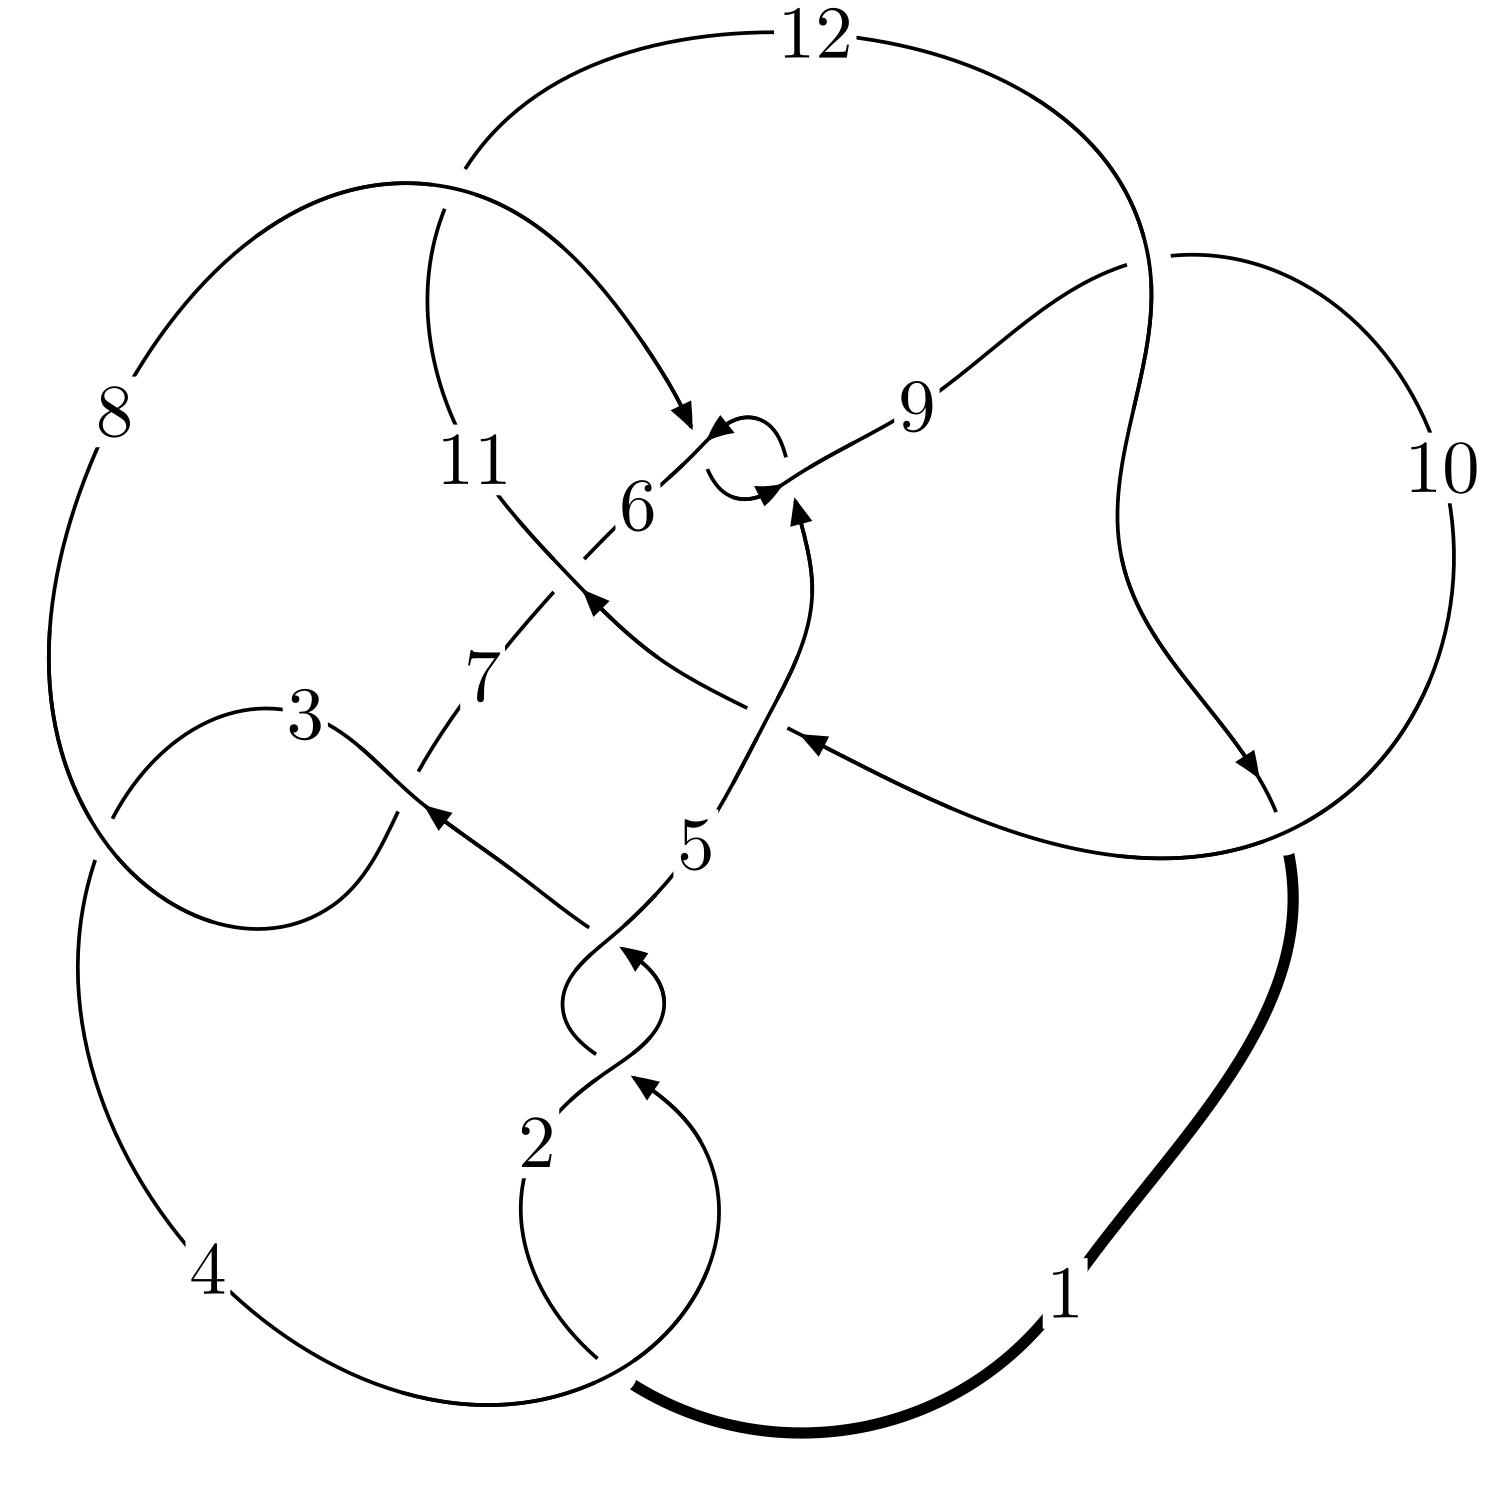
\includegraphics[width=112pt]{../../../GIT/diagram.site/Diagrams/png/2781_12n_0692.png}\\
\ \ \ A knot diagram\footnotemark}&
\allowdisplaybreaks
\textbf{Linearized knot diagam} \\
\cline{2-2}
 &
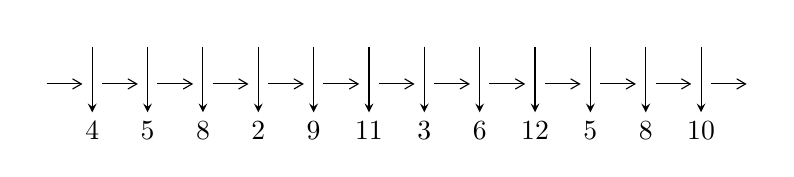
\begin{tikzpicture}[x=20pt, y=17pt]
	% nodes
	\node (C0) at (0, 0) {};
	\node (C1) at (1, 0) {};
	\node (C1U) at (1, +1) {};
	\node (C1D) at (1, -1) {4};

	\node (C2) at (2, 0) {};
	\node (C2U) at (2, +1) {};
	\node (C2D) at (2, -1) {5};

	\node (C3) at (3, 0) {};
	\node (C3U) at (3, +1) {};
	\node (C3D) at (3, -1) {8};

	\node (C4) at (4, 0) {};
	\node (C4U) at (4, +1) {};
	\node (C4D) at (4, -1) {2};

	\node (C5) at (5, 0) {};
	\node (C5U) at (5, +1) {};
	\node (C5D) at (5, -1) {9};

	\node (C6) at (6, 0) {};
	\node (C6U) at (6, +1) {};
	\node (C6D) at (6, -1) {11};

	\node (C7) at (7, 0) {};
	\node (C7U) at (7, +1) {};
	\node (C7D) at (7, -1) {3};

	\node (C8) at (8, 0) {};
	\node (C8U) at (8, +1) {};
	\node (C8D) at (8, -1) {6};

	\node (C9) at (9, 0) {};
	\node (C9U) at (9, +1) {};
	\node (C9D) at (9, -1) {12};

	\node (C10) at (10, 0) {};
	\node (C10U) at (10, +1) {};
	\node (C10D) at (10, -1) {5};

	\node (C11) at (11, 0) {};
	\node (C11U) at (11, +1) {};
	\node (C11D) at (11, -1) {8};

	\node (C12) at (12, 0) {};
	\node (C12U) at (12, +1) {};
	\node (C12D) at (12, -1) {10};
	\node (C13) at (13, 0) {};

	% arrows
	\draw[->,>={angle 60}]
	(C0) edge (C1) (C1) edge (C2) (C2) edge (C3) (C3) edge (C4) (C4) edge (C5) (C5) edge (C6) (C6) edge (C7) (C7) edge (C8) (C8) edge (C9) (C9) edge (C10) (C10) edge (C11) (C11) edge (C12) (C12) edge (C13) ;	\draw[->,>=stealth]
	(C1U) edge (C1D) (C2U) edge (C2D) (C3U) edge (C3D) (C4U) edge (C4D) (C5U) edge (C5D) (C6U) edge (C6D) (C7U) edge (C7D) (C8U) edge (C8D) (C9U) edge (C9D) (C10U) edge (C10D) (C11U) edge (C11D) (C12U) edge (C12D) ;
	\end{tikzpicture} \\
\hhline{~~} \\& 
\textbf{Solving Sequence} \\ \cline{2-2} 
 &
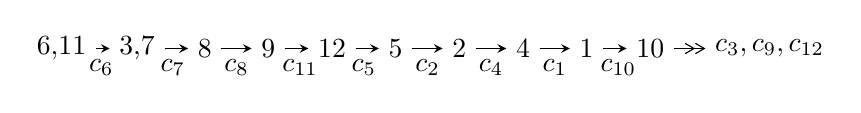
\begin{tikzpicture}[x=23pt, y=7pt]
	% node
	\node (A0) at (-1/8, 0) {6,11};
	\node (A1) at (17/16, 0) {3,7};
	\node (A2) at (17/8, 0) {8};
	\node (A3) at (25/8, 0) {9};
	\node (A4) at (33/8, 0) {12};
	\node (A5) at (41/8, 0) {5};
	\node (A6) at (49/8, 0) {2};
	\node (A7) at (57/8, 0) {4};
	\node (A8) at (65/8, 0) {1};
	\node (A9) at (73/8, 0) {10};
	\node (C1) at (1/2, -1) {$c_{6}$};
	\node (C2) at (13/8, -1) {$c_{7}$};
	\node (C3) at (21/8, -1) {$c_{8}$};
	\node (C4) at (29/8, -1) {$c_{11}$};
	\node (C5) at (37/8, -1) {$c_{5}$};
	\node (C6) at (45/8, -1) {$c_{2}$};
	\node (C7) at (53/8, -1) {$c_{4}$};
	\node (C8) at (61/8, -1) {$c_{1}$};
	\node (C9) at (69/8, -1) {$c_{10}$};
	\node (A10) at (11, 0) {$c_{3},c_{9},c_{12}$};

	% edge
	\draw[->,>=stealth]	
	(A0) edge (A1) (A1) edge (A2) (A2) edge (A3) (A3) edge (A4) (A4) edge (A5) (A5) edge (A6) (A6) edge (A7) (A7) edge (A8) (A8) edge (A9) ;
	\draw[->>,>={angle 60}]	
	(A9) edge (A10);
\end{tikzpicture} \\ 

\end{tabular} \\

\footnotetext{
The image of knot diagram is generated by the software ``\textbf{Draw programme}" developed by Andrew Bartholomew(\url{http://www.layer8.co.uk/maths/draw/index.htm\#Running-draw}), where we modified some parts for our purpose(\url{https://github.com/CATsTAILs/LinksPainter}).
}\phantom \\ \newline 
\centering \textbf{Ideals for irreducible components\footnotemark of $X_{\text{par}}$} 
 
\begin{align*}
I^u_{1}&=\langle 
95253872184 u^{16}+167486372440 u^{15}+\cdots+176471185595 b+60442442928,\\
\phantom{I^u_{1}}&\phantom{= \langle  }-241873986280 u^{16}-181431543352 u^{15}+\cdots+176471185595 a+1319914649856,\\
\phantom{I^u_{1}}&\phantom{= \langle  }u^{17}+u^{16}+\cdots- u-1\rangle \\
I^u_{2}&=\langle 
u^6- u^4+u^2+b+u,\;u^7- u^6- u^5+3 u^4+u^3-3 u^2+a+3,\;u^8- u^7- u^6+2 u^5+u^4-2 u^3+2 u-1\rangle \\
I^u_{3}&=\langle 
4.46740\times10^{15} u^{15}+6.27459\times10^{15} u^{14}+\cdots+2.01298\times10^{18} b-8.81526\times10^{16},\\
\phantom{I^u_{3}}&\phantom{= \langle  }2.12213\times10^{16} u^{15}+2.28177\times10^{16} u^{14}+\cdots+4.02597\times10^{18} a-9.94872\times10^{18},\\
\phantom{I^u_{3}}&\phantom{= \langle  }u^{16}+u^{15}+\cdots-640 u+256\rangle \\
\\
I^v_{1}&=\langle 
a,\;941 v^7+2551 v^6+1791 v^5-6184 v^4-16309 v^3+15249 v^2+887 b+4192 v-1842,\\
\phantom{I^v_{1}}&\phantom{= \langle  }v^8+2 v^7-8 v^5-13 v^4+28 v^3-7 v^2-3 v+1\rangle \\
\end{align*}
\raggedright * 4 irreducible components of $\dim_{\mathbb{C}}=0$, with total 49 representations.\\
\footnotetext{All coefficients of polynomials are rational numbers. But the coefficients are sometimes approximated in decimal forms when there is not enough margin.}
\newpage
\renewcommand{\arraystretch}{1}
\centering \section*{I. $I^u_{1}= \langle 9.53\times10^{10} u^{16}+1.67\times10^{11} u^{15}+\cdots+1.76\times10^{11} b+6.04\times10^{10},\;-2.42\times10^{11} u^{16}-1.81\times10^{11} u^{15}+\cdots+1.76\times10^{11} a+1.32\times10^{12},\;u^{17}+u^{16}+\cdots- u-1 \rangle$}
\flushleft \textbf{(i) Arc colorings}\\
\begin{tabular}{m{7pt} m{180pt} m{7pt} m{180pt} }
\flushright $a_{6}=$&$\begin{pmatrix}1\\0\end{pmatrix}$ \\
\flushright $a_{11}=$&$\begin{pmatrix}0\\u\end{pmatrix}$ \\
\flushright $a_{3}=$&$\begin{pmatrix}1.37061 u^{16}+1.02811 u^{15}+\cdots+7.62117 u-7.47949\\-0.539770 u^{16}-0.949086 u^{15}+\cdots+0.0281086 u-0.342506\end{pmatrix}$ \\
\flushright $a_{7}=$&$\begin{pmatrix}1\\u^2\end{pmatrix}$ \\
\flushright $a_{8}=$&$\begin{pmatrix}0.342506 u^{16}+0.882276 u^{15}+\cdots+6.10888 u-0.370615\\0.409316 u^{16}+0.397625 u^{15}+\cdots+0.882276 u+0.539770\end{pmatrix}$ \\
\flushright $a_{9}=$&$\begin{pmatrix}-0.0668101 u^{16}+0.484651 u^{15}+\cdots+5.22660 u-0.910385\\0.409316 u^{16}+0.397625 u^{15}+\cdots+0.882276 u+0.539770\end{pmatrix}$ \\
\flushright $a_{12}=$&$\begin{pmatrix}1.08601 u^{16}+0.931667 u^{15}+\cdots-6.04983 u-0.704908\\-0.202045 u^{16}-0.0982208 u^{15}+\cdots+0.982581 u-0.563663\end{pmatrix}$ \\
\flushright $a_{5}=$&$\begin{pmatrix}-0.380139 u^{16}-0.473041 u^{15}+\cdots+0.662163 u+1.73660\\-0.183525 u^{16}-0.292667 u^{15}+\cdots-1.16333 u-0.190353\end{pmatrix}$ \\
\flushright $a_{2}=$&$\begin{pmatrix}2.20774 u^{16}+2.09139 u^{15}+\cdots+8.45012 u-9.06872\\-0.720687 u^{16}-0.896329 u^{15}+\cdots+0.887039 u-0.0425575\end{pmatrix}$ \\
\flushright $a_{4}=$&$\begin{pmatrix}1.91038 u^{16}+1.97719 u^{15}+\cdots+7.59306 u-7.13699\\-0.551461 u^{16}-0.673429 u^{15}+\cdots+0.977195 u+0.0668101\end{pmatrix}$ \\
\flushright $a_{1}=$&$\begin{pmatrix}0.301587 u^{16}+0.217988 u^{15}+\cdots+3.13092 u-1.78891\\-0.287349 u^{16}-0.365150 u^{15}+\cdots-0.397625 u+0.0116913\end{pmatrix}$ \\
\flushright $a_{10}=$&$\begin{pmatrix}1.19077 u^{16}+1.37427 u^{15}+\cdots-1.38476 u-1.92738\\-0.0505037 u^{16}+0.0449819 u^{15}+\cdots+1.51534 u-0.116444\end{pmatrix}$\\&\end{tabular}
\flushleft \textbf{(ii) Obstruction class $= -1$}\\~\\
\flushleft \textbf{(iii) Cusp Shapes $= \frac{2048919230872}{176471185595} u^{16}+\frac{1391303845096}{176471185595} u^{15}+\cdots+\frac{3163149744064}{176471185595} u-\frac{6932356318654}{176471185595}$}\\~\\
\newpage\renewcommand{\arraystretch}{1}
\flushleft \textbf{(iv) u-Polynomials at the component}\newline \\
\begin{tabular}{m{50pt}|m{274pt}}
Crossings & \hspace{64pt}u-Polynomials at each crossing \\
\hline $$\begin{aligned}c_{1},c_{2},c_{4}\\c_{9},c_{12}\end{aligned}$$&$\begin{aligned}
&u^{17}-7 u^{16}+\cdots-5 u-1
\end{aligned}$\\
\hline $$\begin{aligned}c_{3},c_{6},c_{7}\end{aligned}$$&$\begin{aligned}
&u^{17}- u^{16}+\cdots- u+1
\end{aligned}$\\
\hline $$\begin{aligned}c_{5},c_{8}\end{aligned}$$&$\begin{aligned}
&u^{17}- u^{16}+\cdots+3 u-1
\end{aligned}$\\
\hline $$\begin{aligned}c_{10}\end{aligned}$$&$\begin{aligned}
&u^{17}+u^{16}+\cdots-699 u+199
\end{aligned}$\\
\hline $$\begin{aligned}c_{11}\end{aligned}$$&$\begin{aligned}
&u^{17}+3 u^{16}+\cdots-263 u-83
\end{aligned}$\\
\hline
\end{tabular}\\~\\
\newpage\renewcommand{\arraystretch}{1}
\flushleft \textbf{(v) Riley Polynomials at the component}\newline \\
\begin{tabular}{m{50pt}|m{274pt}}
Crossings & \hspace{64pt}Riley Polynomials at each crossing \\
\hline $$\begin{aligned}c_{1},c_{2},c_{4}\\c_{9},c_{12}\end{aligned}$$&$\begin{aligned}
&y^{17}-13 y^{16}+\cdots+21 y-1
\end{aligned}$\\
\hline $$\begin{aligned}c_{3},c_{6},c_{7}\end{aligned}$$&$\begin{aligned}
&y^{17}+15 y^{16}+\cdots+13 y-1
\end{aligned}$\\
\hline $$\begin{aligned}c_{5},c_{8}\end{aligned}$$&$\begin{aligned}
&y^{17}+11 y^{16}+\cdots+25 y-1
\end{aligned}$\\
\hline $$\begin{aligned}c_{10}\end{aligned}$$&$\begin{aligned}
&y^{17}+27 y^{16}+\cdots+947097 y-39601
\end{aligned}$\\
\hline $$\begin{aligned}c_{11}\end{aligned}$$&$\begin{aligned}
&y^{17}+7 y^{16}+\cdots+91413 y-6889
\end{aligned}$\\
\hline
\end{tabular}\\~\\
\newpage\flushleft \textbf{(vi) Complex Volumes and Cusp Shapes}
$$\begin{array}{c|c|c}  
\text{Solutions to }I^u_{1}& \I (\text{vol} + \sqrt{-1}CS) & \text{Cusp shape}\\
 \hline 
\begin{aligned}
u &= \phantom{-}0.764077 + 0.442209 I \\
a &= -0.0395160 - 0.1081060 I \\
b &= -0.706366 - 0.510886 I\end{aligned}
 & -4.55533 - 6.93072 I & -21.1582 + 11.9778 I \\ \hline\begin{aligned}
u &= \phantom{-}0.764077 - 0.442209 I \\
a &= -0.0395160 + 0.1081060 I \\
b &= -0.706366 + 0.510886 I\end{aligned}
 & -4.55533 + 6.93072 I & -21.1582 - 11.9778 I \\ \hline\begin{aligned}
u &= -0.791671\phantom{ +0.000000I} \\
a &= \phantom{-}0.0812804\phantom{ +0.000000I} \\
b &= \phantom{-}0.842612\phantom{ +0.000000I}\end{aligned}
 & -8.70952\phantom{ +0.000000I} & -30.7710\phantom{ +0.000000I} \\ \hline\begin{aligned}
u &= \phantom{-}0.753921 + 0.115715 I \\
a &= \phantom{-}2.02750 - 2.62203 I \\
b &= \phantom{-}0.82885 - 1.21720 I\end{aligned}
 & -0.77832 + 2.01331 I & -15.1488 - 1.3786 I \\ \hline\begin{aligned}
u &= \phantom{-}0.753921 - 0.115715 I \\
a &= \phantom{-}2.02750 + 2.62203 I \\
b &= \phantom{-}0.82885 + 1.21720 I\end{aligned}
 & -0.77832 - 2.01331 I & -15.1488 + 1.3786 I \\ \hline\begin{aligned}
u &= -0.502094 + 0.490826 I \\
a &= -0.001938 + 0.710947 I \\
b &= \phantom{-}0.852485 - 0.481916 I\end{aligned}
 & \phantom{-}2.49540 + 2.02523 I & -6.20824 - 3.33819 I \\ \hline\begin{aligned}
u &= -0.502094 - 0.490826 I \\
a &= -0.001938 - 0.710947 I \\
b &= \phantom{-}0.852485 + 0.481916 I\end{aligned}
 & \phantom{-}2.49540 - 2.02523 I & -6.20824 + 3.33819 I \\ \hline\begin{aligned}
u &= -0.291694 + 0.477697 I \\
a &= -2.80059 - 7.96264 I \\
b &= -1.52657 + 1.44231 I\end{aligned}
 & -2.45442 - 0.76114 I & -1.7282 - 15.9915 I \\ \hline\begin{aligned}
u &= -0.291694 - 0.477697 I \\
a &= -2.80059 + 7.96264 I \\
b &= -1.52657 - 1.44231 I\end{aligned}
 & -2.45442 + 0.76114 I & -1.7282 + 15.9915 I \\ \hline\begin{aligned}
u &= \phantom{-}0.439135\phantom{ +0.000000I} \\
a &= \phantom{-}0.660014\phantom{ +0.000000I} \\
b &= -0.311858\phantom{ +0.000000I}\end{aligned}
 & -0.644803\phantom{ +0.000000I} & -15.2830\phantom{ +0.000000I}\\
 \hline 
 \end{array}$$\newpage$$\begin{array}{c|c|c}  
\text{Solutions to }I^u_{1}& \I (\text{vol} + \sqrt{-1}CS) & \text{Cusp shape}\\
 \hline 
\begin{aligned}
u &= -0.432752\phantom{ +0.000000I} \\
a &= -7.32022\phantom{ +0.000000I} \\
b &= -0.938137\phantom{ +0.000000I}\end{aligned}
 & -2.91990\phantom{ +0.000000I} & -47.5300\phantom{ +0.000000I} \\ \hline\begin{aligned}
u &= -0.78485 + 1.87131 I \\
a &= -0.389251 - 0.738414 I \\
b &= -0.26086 + 1.40299 I\end{aligned}
 & \phantom{-}11.20130 + 3.50827 I & -11.32341 - 1.79574 I \\ \hline\begin{aligned}
u &= -0.78485 - 1.87131 I \\
a &= -0.389251 + 0.738414 I \\
b &= -0.26086 - 1.40299 I\end{aligned}
 & \phantom{-}11.20130 - 3.50827 I & -11.32341 + 1.79574 I \\ \hline\begin{aligned}
u &= \phantom{-}0.93651 + 1.91501 I \\
a &= \phantom{-}0.311529 - 0.816594 I \\
b &= \phantom{-}1.12325 + 1.48088 I\end{aligned}
 & \phantom{-}6.80306 - 8.74093 I & -14.7558 + 4.0661 I \\ \hline\begin{aligned}
u &= \phantom{-}0.93651 - 1.91501 I \\
a &= \phantom{-}0.311529 + 0.816594 I \\
b &= \phantom{-}1.12325 - 1.48088 I\end{aligned}
 & \phantom{-}6.80306 + 8.74093 I & -14.7558 - 4.0661 I \\ \hline\begin{aligned}
u &= -0.98322 + 2.02620 I \\
a &= -0.318282 - 0.900844 I \\
b &= -1.60710 + 2.06949 I\end{aligned}
 & \phantom{-}10.6972 + 14.1953 I & -12.00000 - 6.60789 I \\ \hline\begin{aligned}
u &= -0.98322 - 2.02620 I \\
a &= -0.318282 + 0.900844 I \\
b &= -1.60710 - 2.06949 I\end{aligned}
 & \phantom{-}10.6972 - 14.1953 I & -12.00000 + 6.60789 I\\
 \hline 
 \end{array}$$\newpage\newpage\renewcommand{\arraystretch}{1}
\centering \section*{II. $I^u_{2}= \langle u^6- u^4+u^2+b+u,\;u^7- u^6- u^5+3 u^4+u^3-3 u^2+a+3,\;u^8- u^7- u^6+2 u^5+u^4-2 u^3+2 u-1 \rangle$}
\flushleft \textbf{(i) Arc colorings}\\
\begin{tabular}{m{7pt} m{180pt} m{7pt} m{180pt} }
\flushright $a_{6}=$&$\begin{pmatrix}1\\0\end{pmatrix}$ \\
\flushright $a_{11}=$&$\begin{pmatrix}0\\u\end{pmatrix}$ \\
\flushright $a_{3}=$&$\begin{pmatrix}- u^7+u^6+u^5-3 u^4- u^3+3 u^2-3\\- u^6+u^4- u^2- u\end{pmatrix}$ \\
\flushright $a_{7}=$&$\begin{pmatrix}1\\u^2\end{pmatrix}$ \\
\flushright $a_{8}=$&$\begin{pmatrix}1\\u^2\end{pmatrix}$ \\
\flushright $a_{9}=$&$\begin{pmatrix}- u^2+1\\u^2\end{pmatrix}$ \\
\flushright $a_{12}=$&$\begin{pmatrix}- u\\- u^3+u\end{pmatrix}$ \\
\flushright $a_{5}=$&$\begin{pmatrix}u^4- u^2+1\\- u^4\end{pmatrix}$ \\
\flushright $a_{2}=$&$\begin{pmatrix}- u^7+u^6+u^5-4 u^4- u^3+4 u^2-4\\- u^6+2 u^4- u^2- u\end{pmatrix}$ \\
\flushright $a_{4}=$&$\begin{pmatrix}- u^7+u^6+u^5-3 u^4- u^3+3 u^2-3\\- u^6+u^4- u^2- u\end{pmatrix}$ \\
\flushright $a_{1}=$&$\begin{pmatrix}- u^4+u^2-1\\u^4\end{pmatrix}$ \\
\flushright $a_{10}=$&$\begin{pmatrix}- u^6+u^4-2 u^2+1\\- u^7+u^6+2 u^5- u^4-2 u^3+2 u^2+2 u-1\end{pmatrix}$\\&\end{tabular}
\flushleft \textbf{(ii) Obstruction class $= 1$}\\~\\
\flushleft \textbf{(iii) Cusp Shapes $= u^7-4 u^6-2 u^5+5 u^4+3 u^3-5 u^2-5 u-10$}\\~\\
\newpage\renewcommand{\arraystretch}{1}
\flushleft \textbf{(iv) u-Polynomials at the component}\newline \\
\begin{tabular}{m{50pt}|m{274pt}}
Crossings & \hspace{64pt}u-Polynomials at each crossing \\
\hline $$\begin{aligned}c_{1},c_{2}\end{aligned}$$&$\begin{aligned}
&(u-1)^8
\end{aligned}$\\
\hline $$\begin{aligned}c_{3},c_{7}\end{aligned}$$&$\begin{aligned}
&u^8
\end{aligned}$\\
\hline $$\begin{aligned}c_{4}\end{aligned}$$&$\begin{aligned}
&(u+1)^8
\end{aligned}$\\
\hline $$\begin{aligned}c_{5}\end{aligned}$$&$\begin{aligned}
&u^8-3 u^7+7 u^6-10 u^5+11 u^4-10 u^3+6 u^2-4 u+1
\end{aligned}$\\
\hline $$\begin{aligned}c_{6}\end{aligned}$$&$\begin{aligned}
&u^8- u^7- u^6+2 u^5+u^4-2 u^3+2 u-1
\end{aligned}$\\
\hline $$\begin{aligned}c_{8}\end{aligned}$$&$\begin{aligned}
&u^8+3 u^7+7 u^6+10 u^5+11 u^4+10 u^3+6 u^2+4 u+1
\end{aligned}$\\
\hline $$\begin{aligned}c_{9}\end{aligned}$$&$\begin{aligned}
&u^8+u^7-3 u^6-2 u^5+3 u^4+2 u-1
\end{aligned}$\\
\hline $$\begin{aligned}c_{10},c_{12}\end{aligned}$$&$\begin{aligned}
&u^8- u^7-3 u^6+2 u^5+3 u^4-2 u-1
\end{aligned}$\\
\hline $$\begin{aligned}c_{11}\end{aligned}$$&$\begin{aligned}
&u^8+u^7- u^6-2 u^5+u^4+2 u^3-2 u-1
\end{aligned}$\\
\hline
\end{tabular}\\~\\
\newpage\renewcommand{\arraystretch}{1}
\flushleft \textbf{(v) Riley Polynomials at the component}\newline \\
\begin{tabular}{m{50pt}|m{274pt}}
Crossings & \hspace{64pt}Riley Polynomials at each crossing \\
\hline $$\begin{aligned}c_{1},c_{2},c_{4}\end{aligned}$$&$\begin{aligned}
&(y-1)^8
\end{aligned}$\\
\hline $$\begin{aligned}c_{3},c_{7}\end{aligned}$$&$\begin{aligned}
&y^8
\end{aligned}$\\
\hline $$\begin{aligned}c_{5},c_{8}\end{aligned}$$&$\begin{aligned}
&y^8+5 y^7+11 y^6+6 y^5-17 y^4-34 y^3-22 y^2-4 y+1
\end{aligned}$\\
\hline $$\begin{aligned}c_{6},c_{11}\end{aligned}$$&$\begin{aligned}
&y^8-3 y^7+7 y^6-10 y^5+11 y^4-10 y^3+6 y^2-4 y+1
\end{aligned}$\\
\hline $$\begin{aligned}c_{9},c_{10},c_{12}\end{aligned}$$&$\begin{aligned}
&y^8-7 y^7+19 y^6-22 y^5+3 y^4+14 y^3-6 y^2-4 y+1
\end{aligned}$\\
\hline
\end{tabular}\\~\\
\newpage\flushleft \textbf{(vi) Complex Volumes and Cusp Shapes}
$$\begin{array}{c|c|c}  
\text{Solutions to }I^u_{2}& \I (\text{vol} + \sqrt{-1}CS) & \text{Cusp shape}\\
 \hline 
\begin{aligned}
u &= \phantom{-}0.570868 + 0.730671 I \\
a &= -1.21928 + 2.03110 I \\
b &= -1.44082 - 1.43962 I\end{aligned}
 & -2.68559 + 1.13123 I & -18.1377 - 5.3065 I \\ \hline\begin{aligned}
u &= \phantom{-}0.570868 - 0.730671 I \\
a &= -1.21928 - 2.03110 I \\
b &= -1.44082 + 1.43962 I\end{aligned}
 & -2.68559 - 1.13123 I & -18.1377 + 5.3065 I \\ \hline\begin{aligned}
u &= -0.855237 + 0.665892 I \\
a &= \phantom{-}1.230330 + 0.083902 I \\
b &= \phantom{-}0.44992 - 1.37717 I\end{aligned}
 & \phantom{-}0.51448 + 2.57849 I & -10.11893 - 3.45077 I \\ \hline\begin{aligned}
u &= -0.855237 - 0.665892 I \\
a &= \phantom{-}1.230330 - 0.083902 I \\
b &= \phantom{-}0.44992 + 1.37717 I\end{aligned}
 & \phantom{-}0.51448 - 2.57849 I & -10.11893 + 3.45077 I \\ \hline\begin{aligned}
u &= -1.09818\phantom{ +0.000000I} \\
a &= -0.337834\phantom{ +0.000000I} \\
b &= -0.407427\phantom{ +0.000000I}\end{aligned}
 & -8.14766\phantom{ +0.000000I} & -12.9880\phantom{ +0.000000I} \\ \hline\begin{aligned}
u &= \phantom{-}1.031810 + 0.655470 I \\
a &= \phantom{-}0.370895 + 0.073482 I \\
b &= \phantom{-}0.136119 + 0.548347 I\end{aligned}
 & -4.02461 - 6.44354 I & -10.82984 + 2.68172 I \\ \hline\begin{aligned}
u &= \phantom{-}1.031810 - 0.655470 I \\
a &= \phantom{-}0.370895 - 0.073482 I \\
b &= \phantom{-}0.136119 - 0.548347 I\end{aligned}
 & -4.02461 + 6.44354 I & -10.82984 - 2.68172 I \\ \hline\begin{aligned}
u &= \phantom{-}0.603304\phantom{ +0.000000I} \\
a &= -2.42604\phantom{ +0.000000I} \\
b &= -0.883019\phantom{ +0.000000I}\end{aligned}
 & -2.48997\phantom{ +0.000000I} & -13.8390\phantom{ +0.000000I}\\
 \hline 
 \end{array}$$\newpage\newpage\renewcommand{\arraystretch}{1}
\centering \section*{III. $I^u_{3}= \langle 4.47\times10^{15} u^{15}+6.27\times10^{15} u^{14}+\cdots+2.01\times10^{18} b-8.82\times10^{16},\;2.12\times10^{16} u^{15}+2.28\times10^{16} u^{14}+\cdots+4.03\times10^{18} a-9.95\times10^{18},\;u^{16}+u^{15}+\cdots-640 u+256 \rangle$}
\flushleft \textbf{(i) Arc colorings}\\
\begin{tabular}{m{7pt} m{180pt} m{7pt} m{180pt} }
\flushright $a_{6}=$&$\begin{pmatrix}1\\0\end{pmatrix}$ \\
\flushright $a_{11}=$&$\begin{pmatrix}0\\u\end{pmatrix}$ \\
\flushright $a_{3}=$&$\begin{pmatrix}-0.00527110 u^{15}-0.00566765 u^{14}+\cdots-9.23744 u+2.47114\\-0.00221929 u^{15}-0.00311706 u^{14}+\cdots-1.87927 u+0.0437920\end{pmatrix}$ \\
\flushright $a_{7}=$&$\begin{pmatrix}1\\u^2\end{pmatrix}$ \\
\flushright $a_{8}=$&$\begin{pmatrix}0.00131807 u^{15}-0.000965283 u^{14}+\cdots+5.02090 u-2.85900\\0.00125266 u^{15}+0.00142411 u^{14}+\cdots+2.92217 u-0.895088\end{pmatrix}$ \\
\flushright $a_{9}=$&$\begin{pmatrix}0.0000654109 u^{15}-0.00238940 u^{14}+\cdots+2.09873 u-1.96392\\0.00125266 u^{15}+0.00142411 u^{14}+\cdots+2.92217 u-0.895088\end{pmatrix}$ \\
\flushright $a_{12}=$&$\begin{pmatrix}0.000844467 u^{15}-0.00179388 u^{14}+\cdots+1.76050 u-2.43832\\0.000597578 u^{15}+0.000131722 u^{14}+\cdots+3.26843 u-1.14785\end{pmatrix}$ \\
\flushright $a_{5}=$&$\begin{pmatrix}0.00355246 u^{15}+0.00420683 u^{14}+\cdots+4.56085 u+0.0559940\\0.000931308 u^{15}+0.000874523 u^{14}+\cdots+1.47705 u+0.342822\end{pmatrix}$ \\
\flushright $a_{2}=$&$\begin{pmatrix}-0.00941161 u^{15}-0.0110390 u^{14}+\cdots-13.9929 u+1.68523\\-0.00326781 u^{15}-0.00500207 u^{14}+\cdots-3.20051 u-0.587143\end{pmatrix}$ \\
\flushright $a_{4}=$&$\begin{pmatrix}-0.00749346 u^{15}-0.00988307 u^{14}+\cdots-11.5790 u+0.607025\\-0.00129900 u^{15}-0.00377384 u^{14}+\cdots-0.399220 u-1.24590\end{pmatrix}$ \\
\flushright $a_{1}=$&$\begin{pmatrix}-0.00155963 u^{15}+0.00229520 u^{14}+\cdots-2.60619 u+2.70441\\-0.00272297 u^{15}-0.00333262 u^{14}+\cdots-4.50999 u+1.52352\end{pmatrix}$ \\
\flushright $a_{10}=$&$\begin{pmatrix}-0.0000400338 u^{15}-0.00236158 u^{14}+\cdots+0.837916 u-1.48462\\0.000345643 u^{15}-0.00112847 u^{14}+\cdots+1.97094 u-0.673787\end{pmatrix}$\\&\end{tabular}
\flushleft \textbf{(ii) Obstruction class $= -1$}\\~\\
\flushleft \textbf{(iii) Cusp Shapes $= -\frac{4129940980039711}{1006491371550221696} u^{15}-\frac{3800282985571637}{1006491371550221696} u^{14}+\cdots-\frac{45304359399533900}{7863213840236107} u-\frac{73541352487366340}{7863213840236107}$}\\~\\
\newpage\renewcommand{\arraystretch}{1}
\flushleft \textbf{(iv) u-Polynomials at the component}\newline \\
\begin{tabular}{m{50pt}|m{274pt}}
Crossings & \hspace{64pt}u-Polynomials at each crossing \\
\hline $$\begin{aligned}c_{1},c_{2},c_{4}\\c_{9},c_{12}\end{aligned}$$&$\begin{aligned}
&u^{16}-3 u^{15}+\cdots-8 u+1
\end{aligned}$\\
\hline $$\begin{aligned}c_{3},c_{6},c_{7}\end{aligned}$$&$\begin{aligned}
&u^{16}- u^{15}+\cdots+640 u+256
\end{aligned}$\\
\hline $$\begin{aligned}c_{5},c_{8}\end{aligned}$$&$\begin{aligned}
&(u^8- u^7+3 u^6-2 u^5+3 u^4-2 u^3-1)^2
\end{aligned}$\\
\hline $$\begin{aligned}c_{10}\end{aligned}$$&$\begin{aligned}
&u^{16}+3 u^{15}+\cdots+2169 u+361
\end{aligned}$\\
\hline $$\begin{aligned}c_{11}\end{aligned}$$&$\begin{aligned}
&u^{16}-4 u^{15}+\cdots-189 u+297
\end{aligned}$\\
\hline
\end{tabular}\\~\\
\newpage\renewcommand{\arraystretch}{1}
\flushleft \textbf{(v) Riley Polynomials at the component}\newline \\
\begin{tabular}{m{50pt}|m{274pt}}
Crossings & \hspace{64pt}Riley Polynomials at each crossing \\
\hline $$\begin{aligned}c_{1},c_{2},c_{4}\\c_{9},c_{12}\end{aligned}$$&$\begin{aligned}
&y^{16}+9 y^{15}+\cdots+4 y+1
\end{aligned}$\\
\hline $$\begin{aligned}c_{3},c_{6},c_{7}\end{aligned}$$&$\begin{aligned}
&y^{16}+33 y^{15}+\cdots+606208 y+65536
\end{aligned}$\\
\hline $$\begin{aligned}c_{5},c_{8}\end{aligned}$$&$\begin{aligned}
&(y^8+5 y^7+11 y^6+10 y^5- y^4-10 y^3-6 y^2+1)^2
\end{aligned}$\\
\hline $$\begin{aligned}c_{10}\end{aligned}$$&$\begin{aligned}
&y^{16}+31 y^{15}+\cdots-741503 y+130321
\end{aligned}$\\
\hline $$\begin{aligned}c_{11}\end{aligned}$$&$\begin{aligned}
&y^{16}+32 y^{15}+\cdots+78327 y+88209
\end{aligned}$\\
\hline
\end{tabular}\\~\\
\newpage\flushleft \textbf{(vi) Complex Volumes and Cusp Shapes}
$$\begin{array}{c|c|c}  
\text{Solutions to }I^u_{3}& \I (\text{vol} + \sqrt{-1}CS) & \text{Cusp shape}\\
 \hline 
\begin{aligned}
u &= \phantom{-}0.928106 + 0.575657 I \\
a &= \phantom{-}0.314063 - 0.194797 I \\
b &= -0.553504 + 0.808003 I\end{aligned}
 & -0.290648\phantom{ +0.000000I} & -13.26997 + 0. I\phantom{ +0.000000I} \\ \hline\begin{aligned}
u &= \phantom{-}0.928106 - 0.575657 I \\
a &= \phantom{-}0.314063 + 0.194797 I \\
b &= -0.553504 - 0.808003 I\end{aligned}
 & -0.290648\phantom{ +0.000000I} & -13.26997 + 0. I\phantom{ +0.000000I} \\ \hline\begin{aligned}
u &= \phantom{-}0.684023 + 0.882805 I \\
a &= \phantom{-}0.471554 - 0.908141 I \\
b &= \phantom{-}0.796152 + 0.451692 I\end{aligned}
 & -1.15366 + 1.27532 I & -10.53127 - 1.72199 I \\ \hline\begin{aligned}
u &= \phantom{-}0.684023 - 0.882805 I \\
a &= \phantom{-}0.471554 + 0.908141 I \\
b &= \phantom{-}0.796152 - 0.451692 I\end{aligned}
 & -1.15366 - 1.27532 I & -10.53127 + 1.72199 I \\ \hline\begin{aligned}
u &= -0.577755 + 0.986475 I \\
a &= \phantom{-}0.367269 - 0.263106 I \\
b &= \phantom{-}1.083960 + 0.732960 I\end{aligned}
 & \phantom{-}2.70026 - 3.63283 I & -9.34305 + 4.59352 I \\ \hline\begin{aligned}
u &= -0.577755 - 0.986475 I \\
a &= \phantom{-}0.367269 + 0.263106 I \\
b &= \phantom{-}1.083960 - 0.732960 I\end{aligned}
 & \phantom{-}2.70026 + 3.63283 I & -9.34305 - 4.59352 I \\ \hline\begin{aligned}
u &= \phantom{-}0.153757 + 0.400659 I \\
a &= \phantom{-}0.49286 - 2.61690 I \\
b &= -0.429065 - 0.463862 I\end{aligned}
 & -1.15366 + 1.27532 I & -10.53127 - 1.72199 I \\ \hline\begin{aligned}
u &= \phantom{-}0.153757 - 0.400659 I \\
a &= \phantom{-}0.49286 + 2.61690 I \\
b &= -0.429065 + 0.463862 I\end{aligned}
 & -1.15366 - 1.27532 I & -10.53127 + 1.72199 I \\ \hline\begin{aligned}
u &= -1.61868 + 0.98339 I \\
a &= -0.162363 + 0.219097 I \\
b &= \phantom{-}1.00687 + 1.86555 I\end{aligned}
 & \phantom{-}2.70026 + 3.63283 I & -9.34305 - 4.59352 I \\ \hline\begin{aligned}
u &= -1.61868 - 0.98339 I \\
a &= -0.162363 - 0.219097 I \\
b &= \phantom{-}1.00687 - 1.86555 I\end{aligned}
 & \phantom{-}2.70026 - 3.63283 I & -9.34305 + 4.59352 I\\
 \hline 
 \end{array}$$\newpage$$\begin{array}{c|c|c}  
\text{Solutions to }I^u_{3}& \I (\text{vol} + \sqrt{-1}CS) & \text{Cusp shape}\\
 \hline 
\begin{aligned}
u &= -0.05666 + 2.24811 I \\
a &= -0.079508 + 0.874899 I \\
b &= \phantom{-}0.48785 - 1.75982 I\end{aligned}
 & \phantom{-}12.42750 + 4.93524 I & -10.31351 - 3.19667 I \\ \hline\begin{aligned}
u &= -0.05666 - 2.24811 I \\
a &= -0.079508 - 0.874899 I \\
b &= \phantom{-}0.48785 + 1.75982 I\end{aligned}
 & \phantom{-}12.42750 - 4.93524 I & -10.31351 + 3.19667 I \\ \hline\begin{aligned}
u &= -0.14941 + 2.37106 I \\
a &= \phantom{-}0.048233 + 0.765446 I \\
b &= \phantom{-}0.42164 - 1.94931 I\end{aligned}
 & \phantom{-}8.53095\phantom{ +0.000000I} & -13.35437 + 0. I\phantom{ +0.000000I} \\ \hline\begin{aligned}
u &= -0.14941 - 2.37106 I \\
a &= \phantom{-}0.048233 - 0.765446 I \\
b &= \phantom{-}0.42164 + 1.94931 I\end{aligned}
 & \phantom{-}8.53095\phantom{ +0.000000I} & -13.35437 + 0. I\phantom{ +0.000000I} \\ \hline\begin{aligned}
u &= \phantom{-}0.13661 + 2.63887 I \\
a &= \phantom{-}0.047894 + 0.746119 I \\
b &= -0.81390 - 2.89913 I\end{aligned}
 & \phantom{-}12.42750 - 4.93524 I & -10.31351 + 3.19667 I \\ \hline\begin{aligned}
u &= \phantom{-}0.13661 - 2.63887 I \\
a &= \phantom{-}0.047894 - 0.746119 I \\
b &= -0.81390 + 2.89913 I\end{aligned}
 & \phantom{-}12.42750 + 4.93524 I & -10.31351 - 3.19667 I\\
 \hline 
 \end{array}$$\newpage\newpage\renewcommand{\arraystretch}{1}
\centering \section*{IV. $I^v_{1}= \langle a,\;941 v^7+2551 v^6+\cdots+887 b-1842,\;v^8+2 v^7-8 v^5-13 v^4+28 v^3-7 v^2-3 v+1 \rangle$}
\flushleft \textbf{(i) Arc colorings}\\
\begin{tabular}{m{7pt} m{180pt} m{7pt} m{180pt} }
\flushright $a_{6}=$&$\begin{pmatrix}1\\0\end{pmatrix}$ \\
\flushright $a_{11}=$&$\begin{pmatrix}v\\0\end{pmatrix}$ \\
\flushright $a_{3}=$&$\begin{pmatrix}0\\-1.06088 v^{7}-2.87599 v^{6}+\cdots-4.72604 v+2.07666\end{pmatrix}$ \\
\flushright $a_{7}=$&$\begin{pmatrix}1\\0\end{pmatrix}$ \\
\flushright $a_{8}=$&$\begin{pmatrix}1\\1.62683 v^{7}+3.57497 v^{6}+\cdots+1.17926 v-3.82638\end{pmatrix}$ \\
\flushright $a_{9}=$&$\begin{pmatrix}-1.62683 v^{7}-3.57497 v^{6}+\cdots-1.17926 v+4.82638\\1.62683 v^{7}+3.57497 v^{6}+\cdots+1.17926 v-3.82638\end{pmatrix}$ \\
\flushright $a_{12}=$&$\begin{pmatrix}0.321308 v^{7}+0.456595 v^{6}+\cdots+2.05411 v-1.62683\\0.568207 v^{7}+1.17587 v^{6}+\cdots+0.443067 v-2.38219\end{pmatrix}$ \\
\flushright $a_{5}=$&$\begin{pmatrix}0.755355 v^{7}+1.75761 v^{6}+\cdots-2.39910 v-1.87711\\-2.38219 v^{7}-5.33258 v^{6}+\cdots+1.21984 v+6.70349\end{pmatrix}$ \\
\flushright $a_{2}=$&$\begin{pmatrix}0.244645 v^{7}+0.242390 v^{6}+\cdots-4.60090 v-1.12289\\-3.44419 v^{7}-7.94701 v^{6}+\cdots-1.00113 v+9.59639\end{pmatrix}$ \\
\flushright $a_{4}=$&$\begin{pmatrix}1.06088 v^{7}+2.87599 v^{6}+\cdots+4.72604 v-2.07666\\1.57046 v^{7}+3.65276 v^{6}+\cdots+0.432920 v-5.01466\end{pmatrix}$ \\
\flushright $a_{1}=$&$\begin{pmatrix}1.62683 v^{7}+3.57497 v^{6}+\cdots+1.17926 v-4.82638\\-1.62683 v^{7}-3.57497 v^{6}+\cdots-1.17926 v+3.82638\end{pmatrix}$ \\
\flushright $a_{10}=$&$\begin{pmatrix}-1.30552 v^{7}-3.11838 v^{6}+\cdots+0.874859 v+3.19955\\2.19504 v^{7}+4.75085 v^{6}+\cdots+1.62232 v-6.20857\end{pmatrix}$\\&\end{tabular}
\flushleft \textbf{(ii) Obstruction class $= 1$}\\~\\
\flushleft \textbf{(iii) Cusp Shapes $= \frac{2247}{887} v^7+\frac{4687}{887} v^6-\frac{426}{887} v^5-\frac{21184}{887} v^4-\frac{35807}{887} v^3+\frac{61378}{887} v^2+\frac{5411}{887} v-\frac{17810}{887}$}\\~\\
\newpage\renewcommand{\arraystretch}{1}
\flushleft \textbf{(iv) u-Polynomials at the component}\newline \\
\begin{tabular}{m{50pt}|m{274pt}}
Crossings & \hspace{64pt}u-Polynomials at each crossing \\
\hline $$\begin{aligned}c_{1},c_{2}\end{aligned}$$&$\begin{aligned}
&u^8+u^7-3 u^6-2 u^5+3 u^4+2 u-1
\end{aligned}$\\
\hline $$\begin{aligned}c_{3}\end{aligned}$$&$\begin{aligned}
&u^8- u^7- u^6+2 u^5+u^4-2 u^3+2 u-1
\end{aligned}$\\
\hline $$\begin{aligned}c_{4}\end{aligned}$$&$\begin{aligned}
&u^8- u^7-3 u^6+2 u^5+3 u^4-2 u-1
\end{aligned}$\\
\hline $$\begin{aligned}c_{5}\end{aligned}$$&$\begin{aligned}
&u^8-3 u^7+7 u^6-10 u^5+11 u^4-10 u^3+6 u^2-4 u+1
\end{aligned}$\\
\hline $$\begin{aligned}c_{6}\end{aligned}$$&$\begin{aligned}
&u^8
\end{aligned}$\\
\hline $$\begin{aligned}c_{7}\end{aligned}$$&$\begin{aligned}
&u^8+u^7- u^6-2 u^5+u^4+2 u^3-2 u-1
\end{aligned}$\\
\hline $$\begin{aligned}c_{8}\end{aligned}$$&$\begin{aligned}
&u^8+3 u^7+7 u^6+10 u^5+11 u^4+10 u^3+6 u^2+4 u+1
\end{aligned}$\\
\hline $$\begin{aligned}c_{9}\end{aligned}$$&$\begin{aligned}
&(u-1)^8
\end{aligned}$\\
\hline $$\begin{aligned}c_{10}\end{aligned}$$&$\begin{aligned}
&u^8-2 u^7- u^6+5 u^5+4 u^4-17 u^3+17 u^2-7 u+1
\end{aligned}$\\
\hline $$\begin{aligned}c_{11}\end{aligned}$$&$\begin{aligned}
&u^8+3 u^7+6 u^6+7 u^5+13 u^4+11 u^3+4 u^2+3 u+1
\end{aligned}$\\
\hline $$\begin{aligned}c_{12}\end{aligned}$$&$\begin{aligned}
&(u+1)^8
\end{aligned}$\\
\hline
\end{tabular}\\~\\
\newpage\renewcommand{\arraystretch}{1}
\flushleft \textbf{(v) Riley Polynomials at the component}\newline \\
\begin{tabular}{m{50pt}|m{274pt}}
Crossings & \hspace{64pt}Riley Polynomials at each crossing \\
\hline $$\begin{aligned}c_{1},c_{2},c_{4}\end{aligned}$$&$\begin{aligned}
&y^8-7 y^7+19 y^6-22 y^5+3 y^4+14 y^3-6 y^2-4 y+1
\end{aligned}$\\
\hline $$\begin{aligned}c_{3},c_{7}\end{aligned}$$&$\begin{aligned}
&y^8-3 y^7+7 y^6-10 y^5+11 y^4-10 y^3+6 y^2-4 y+1
\end{aligned}$\\
\hline $$\begin{aligned}c_{5},c_{8}\end{aligned}$$&$\begin{aligned}
&y^8+5 y^7+11 y^6+6 y^5-17 y^4-34 y^3-22 y^2-4 y+1
\end{aligned}$\\
\hline $$\begin{aligned}c_{6}\end{aligned}$$&$\begin{aligned}
&y^8
\end{aligned}$\\
\hline $$\begin{aligned}c_{9},c_{12}\end{aligned}$$&$\begin{aligned}
&(y-1)^8
\end{aligned}$\\
\hline $$\begin{aligned}c_{10}\end{aligned}$$&$\begin{aligned}
&y^8-6 y^7+29 y^6-67 y^5+126 y^4-85 y^3+59 y^2-15 y+1
\end{aligned}$\\
\hline $$\begin{aligned}c_{11}\end{aligned}$$&$\begin{aligned}
&y^8+3 y^7+20 y^6+49 y^5+47 y^4-47 y^3-24 y^2- y+1
\end{aligned}$\\
\hline
\end{tabular}\\~\\
\newpage\flushleft \textbf{(vi) Complex Volumes and Cusp Shapes}
$$\begin{array}{c|c|c}  
\text{Solutions to }I^v_{1}& \I (\text{vol} + \sqrt{-1}CS) & \text{Cusp shape}\\
 \hline 
\begin{aligned}
v &= \phantom{-}1.230330 + 0.083902 I \\
a &= \phantom{-0.000000 } 0 \\
b &= \phantom{-}0.855237 - 0.665892 I\end{aligned}
 & \phantom{-}0.51448 + 2.57849 I & -10.11893 - 3.45077 I \\ \hline\begin{aligned}
v &= \phantom{-}1.230330 - 0.083902 I \\
a &= \phantom{-0.000000 } 0 \\
b &= \phantom{-}0.855237 + 0.665892 I\end{aligned}
 & \phantom{-}0.51448 - 2.57849 I & -10.11893 + 3.45077 I \\ \hline\begin{aligned}
v &= \phantom{-}0.370895 + 0.073482 I \\
a &= \phantom{-0.000000 } 0 \\
b &= -1.031810 - 0.655470 I\end{aligned}
 & -4.02461 - 6.44354 I & -10.82984 + 2.68172 I \\ \hline\begin{aligned}
v &= \phantom{-}0.370895 - 0.073482 I \\
a &= \phantom{-0.000000 } 0 \\
b &= -1.031810 + 0.655470 I\end{aligned}
 & -4.02461 + 6.44354 I & -10.82984 - 2.68172 I \\ \hline\begin{aligned}
v &= -0.337834\phantom{ +0.000000I} \\
a &= \phantom{-0.000000 } 0 \\
b &= \phantom{-}1.09818\phantom{ +0.000000I}\end{aligned}
 & -8.14766\phantom{ +0.000000I} & -12.9880\phantom{ +0.000000I} \\ \hline\begin{aligned}
v &= -1.21928 + 2.03110 I \\
a &= \phantom{-0.000000 } 0 \\
b &= -0.570868 - 0.730671 I\end{aligned}
 & -2.68559 + 1.13123 I & -18.1377 - 5.3065 I \\ \hline\begin{aligned}
v &= -1.21928 - 2.03110 I \\
a &= \phantom{-0.000000 } 0 \\
b &= -0.570868 + 0.730671 I\end{aligned}
 & -2.68559 - 1.13123 I & -18.1377 + 5.3065 I \\ \hline\begin{aligned}
v &= -2.42604\phantom{ +0.000000I} \\
a &= \phantom{-0.000000 } 0 \\
b &= -0.603304\phantom{ +0.000000I}\end{aligned}
 & -2.48997\phantom{ +0.000000I} & -13.8390\phantom{ +0.000000I}\\
 \hline 
 \end{array}$$\newpage
\newpage\renewcommand{\arraystretch}{1}
\centering \section*{ V. u-Polynomials}
\begin{tabular}{m{50pt}|m{274pt}}
Crossings & \hspace{64pt}u-Polynomials at each crossing \\
\hline $$\begin{aligned}c_{1},c_{2},c_{9}\end{aligned}$$&$\begin{aligned}
&((u-1)^8)(u^8+u^7+\cdots+2 u-1)(u^{16}-3 u^{15}+\cdots-8 u+1)\\
&\cdot(u^{17}-7 u^{16}+\cdots-5 u-1)
\end{aligned}$\\
\hline $$\begin{aligned}c_{3},c_{6}\end{aligned}$$&$\begin{aligned}
&u^8(u^8- u^7+\cdots+2 u-1)(u^{16}- u^{15}+\cdots+640 u+256)\\
&\cdot(u^{17}- u^{16}+\cdots- u+1)
\end{aligned}$\\
\hline $$\begin{aligned}c_{4},c_{12}\end{aligned}$$&$\begin{aligned}
&((u+1)^8)(u^8- u^7+\cdots-2 u-1)(u^{16}-3 u^{15}+\cdots-8 u+1)\\
&\cdot(u^{17}-7 u^{16}+\cdots-5 u-1)
\end{aligned}$\\
\hline $$\begin{aligned}c_{5}\end{aligned}$$&$\begin{aligned}
&(u^8-3 u^7+7 u^6-10 u^5+11 u^4-10 u^3+6 u^2-4 u+1)^2\\
&\cdot((u^8- u^7+\cdots-2 u^3-1)^{2})(u^{17}- u^{16}+\cdots+3 u-1)
\end{aligned}$\\
\hline $$\begin{aligned}c_{7}\end{aligned}$$&$\begin{aligned}
&u^8(u^8+u^7+\cdots-2 u-1)(u^{16}- u^{15}+\cdots+640 u+256)\\
&\cdot(u^{17}- u^{16}+\cdots- u+1)
\end{aligned}$\\
\hline $$\begin{aligned}c_{8}\end{aligned}$$&$\begin{aligned}
&(u^8- u^7+3 u^6-2 u^5+3 u^4-2 u^3-1)^2\\
&\cdot(u^8+3 u^7+7 u^6+10 u^5+11 u^4+10 u^3+6 u^2+4 u+1)^2\\
&\cdot(u^{17}- u^{16}+\cdots+3 u-1)
\end{aligned}$\\
\hline $$\begin{aligned}c_{10}\end{aligned}$$&$\begin{aligned}
&(u^8-2 u^7- u^6+5 u^5+4 u^4-17 u^3+17 u^2-7 u+1)\\
&\cdot(u^8- u^7-3 u^6+2 u^5+3 u^4-2 u-1)(u^{16}+3 u^{15}+\cdots+2169 u+361)\\
&\cdot(u^{17}+u^{16}+\cdots-699 u+199)
\end{aligned}$\\
\hline $$\begin{aligned}c_{11}\end{aligned}$$&$\begin{aligned}
&(u^8+u^7- u^6-2 u^5+u^4+2 u^3-2 u-1)\\
&\cdot(u^8+3 u^7+6 u^6+7 u^5+13 u^4+11 u^3+4 u^2+3 u+1)\\
&\cdot(u^{16}-4 u^{15}+\cdots-189 u+297)(u^{17}+3 u^{16}+\cdots-263 u-83)
\end{aligned}$\\
\hline
\end{tabular}\newpage\renewcommand{\arraystretch}{1}
\centering \section*{ VI. Riley Polynomials}
\begin{tabular}{m{50pt}|m{274pt}}
Crossings & \hspace{64pt}Riley Polynomials at each crossing \\
\hline $$\begin{aligned}c_{1},c_{2},c_{4}\\c_{9},c_{12}\end{aligned}$$&$\begin{aligned}
&(y-1)^8(y^8-7 y^7+19 y^6-22 y^5+3 y^4+14 y^3-6 y^2-4 y+1)\\
&\cdot(y^{16}+9 y^{15}+\cdots+4 y+1)(y^{17}-13 y^{16}+\cdots+21 y-1)
\end{aligned}$\\
\hline $$\begin{aligned}c_{3},c_{6},c_{7}\end{aligned}$$&$\begin{aligned}
&y^8(y^8-3 y^7+7 y^6-10 y^5+11 y^4-10 y^3+6 y^2-4 y+1)\\
&\cdot(y^{16}+33 y^{15}+\cdots+606208 y+65536)(y^{17}+15 y^{16}+\cdots+13 y-1)
\end{aligned}$\\
\hline $$\begin{aligned}c_{5},c_{8}\end{aligned}$$&$\begin{aligned}
&(y^8+5 y^7+11 y^6+6 y^5-17 y^4-34 y^3-22 y^2-4 y+1)^2\\
&\cdot(y^8+5 y^7+11 y^6+10 y^5- y^4-10 y^3-6 y^2+1)^2\\
&\cdot(y^{17}+11 y^{16}+\cdots+25 y-1)
\end{aligned}$\\
\hline $$\begin{aligned}c_{10}\end{aligned}$$&$\begin{aligned}
&(y^8-7 y^7+19 y^6-22 y^5+3 y^4+14 y^3-6 y^2-4 y+1)\\
&\cdot(y^8-6 y^7+29 y^6-67 y^5+126 y^4-85 y^3+59 y^2-15 y+1)\\
&\cdot(y^{16}+31 y^{15}+\cdots-741503 y+130321)\\
&\cdot(y^{17}+27 y^{16}+\cdots+947097 y-39601)
\end{aligned}$\\
\hline $$\begin{aligned}c_{11}\end{aligned}$$&$\begin{aligned}
&(y^8-3 y^7+7 y^6-10 y^5+11 y^4-10 y^3+6 y^2-4 y+1)\\
&\cdot(y^8+3 y^7+20 y^6+49 y^5+47 y^4-47 y^3-24 y^2- y+1)\\
&\cdot(y^{16}+32 y^{15}+\cdots+78327 y+88209)\\
&\cdot(y^{17}+7 y^{16}+\cdots+91413 y-6889)
\end{aligned}$\\
\hline
\end{tabular}
\vskip 2pc
\end{document}